\documentclass{standalone}
\usepackage{tikz}
\usetikzlibrary{patterns, positioning}
\usepackage[sfdefault]{ClearSans} %% option 'sfdefault' activates Clear Sans as the default text font
\usepackage[T1]{fontenc}

\begin{document}
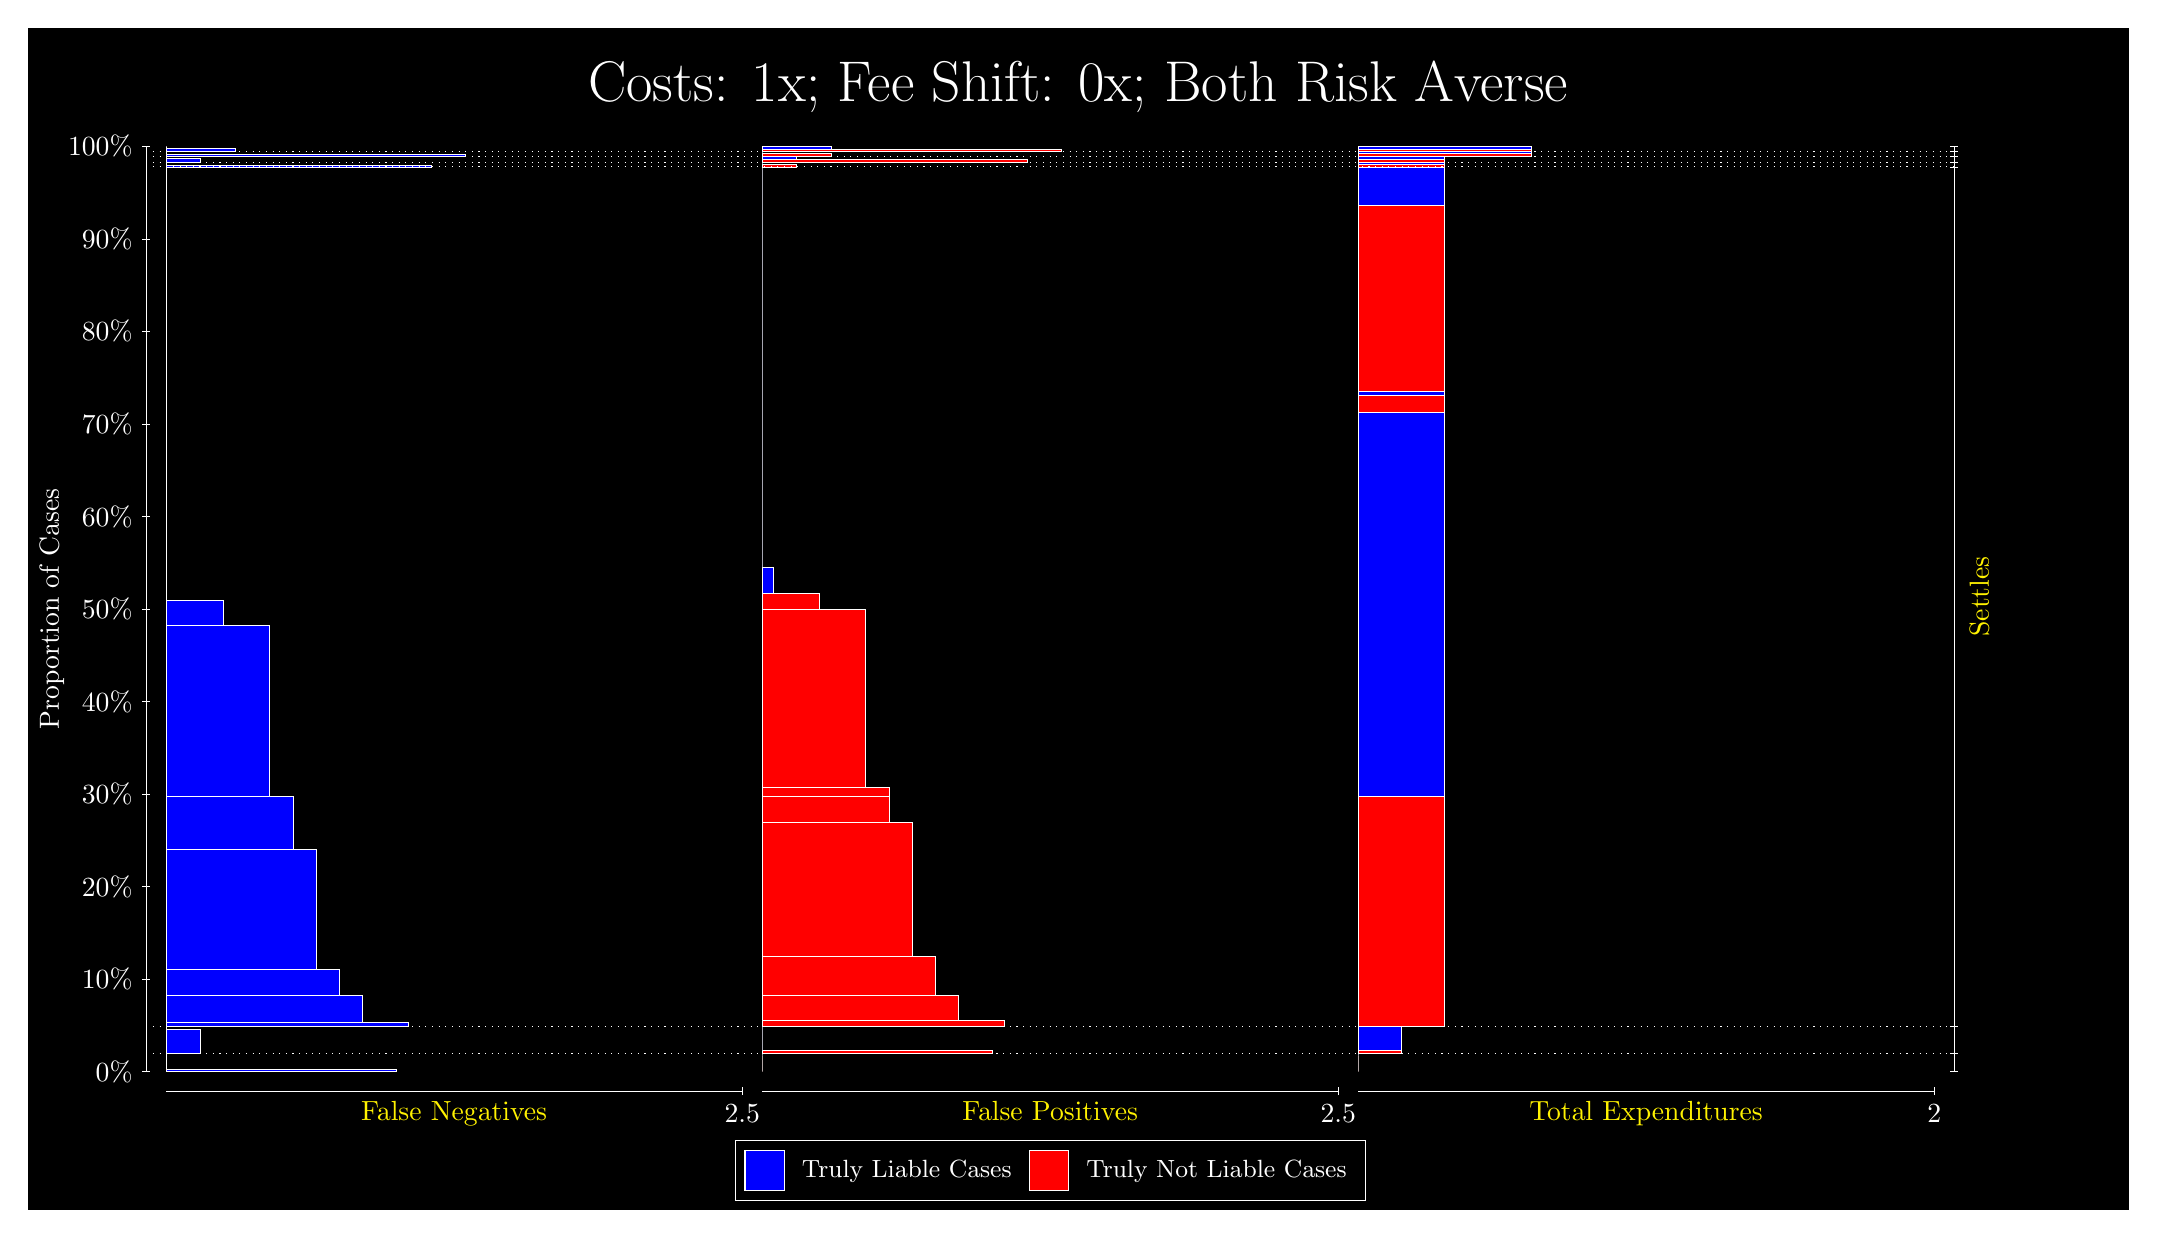
\begin{tikzpicture}
\draw[fill=black] (0,0) rectangle (26.667,15);
\draw[text=white] (0,13.5) rectangle (26.667,15) node[midway] {\huge Costs: 1x; Fee Shift: 0x; Both Risk Averse};
\draw[white, very thin] (1.5,1.75) -- (1.5,13.5);
\node[rotate=90, text=white, anchor=center] at (0.3, 7.625) {Proportion of Cases};
\draw[white, very thin] (1.45,1.75) -- (1.55,1.75);
\node[text=white, anchor=east] at (1.45, 1.75) {0\%};
\draw[white, very thin] (1.45,2.925) -- (1.55,2.925);
\node[text=white, anchor=east] at (1.45, 2.925) {10\%};
\draw[white, very thin] (1.45,4.1) -- (1.55,4.1);
\node[text=white, anchor=east] at (1.45, 4.1) {20\%};
\draw[white, very thin] (1.45,5.275) -- (1.55,5.275);
\node[text=white, anchor=east] at (1.45, 5.275) {30\%};
\draw[white, very thin] (1.45,6.45) -- (1.55,6.45);
\node[text=white, anchor=east] at (1.45, 6.45) {40\%};
\draw[white, very thin] (1.45,7.625) -- (1.55,7.625);
\node[text=white, anchor=east] at (1.45, 7.625) {50\%};
\draw[white, very thin] (1.45,8.8) -- (1.55,8.8);
\node[text=white, anchor=east] at (1.45, 8.8) {60\%};
\draw[white, very thin] (1.45,9.975) -- (1.55,9.975);
\node[text=white, anchor=east] at (1.45, 9.975) {70\%};
\draw[white, very thin] (1.45,11.15) -- (1.55,11.15);
\node[text=white, anchor=east] at (1.45, 11.15) {80\%};
\draw[white, very thin] (1.45,12.325) -- (1.55,12.325);
\node[text=white, anchor=east] at (1.45, 12.325) {90\%};
\draw[white, very thin] (1.45,13.5) -- (1.55,13.5);
\node[text=white, anchor=east] at (1.45, 13.5) {100\%};

\draw[white, very thin] (24.457,1.75) -- (24.457,13.5);
\draw[white, very thin] (24.407,1.75) -- (24.507,1.75);
\node[anchor=west] at (24.407, 1.75) {};
\draw[white, very thin] (24.407,1.9801) -- (24.507,1.9801);
\node[anchor=west] at (24.407, 1.9801) {};
\draw[white, very thin] (24.407,2.3253) -- (24.507,2.3253);
\node[anchor=west] at (24.407, 2.3253) {};
\draw[white, very thin] (24.407,13.24) -- (24.507,13.24);
\node[anchor=west] at (24.407, 13.24) {};
\draw[white, very thin] (24.407,13.297) -- (24.507,13.297);
\node[anchor=west] at (24.407, 13.297) {};
\draw[white, very thin] (24.407,13.375) -- (24.507,13.375);
\node[anchor=west] at (24.407, 13.375) {};
\draw[white, very thin] (24.407,13.439) -- (24.507,13.439);
\node[anchor=west] at (24.407, 13.439) {};
\draw[white, very thin] (24.407,13.5) -- (24.507,13.5);
\node[anchor=west] at (24.407, 13.5) {};

\draw[white, very thin, fill=blue] (1.75,1.75) rectangle (4.6775,1.7742);
\draw[white, very thin, fill=red] (1.75,1.7742) rectangle (1.75,1.9801);
\draw[white, very thin, fill=blue] (1.75,1.9801) rectangle (2.1891,2.289);
\draw[white, very thin, fill=red] (1.75,2.289) rectangle (1.75,2.3253);
\draw[white, very thin, fill=blue] (1.75,2.3253) rectangle (4.8239,2.3724);
\draw[white, very thin, fill=blue] (1.75,2.3724) rectangle (4.2384,2.7197);
\draw[white, very thin, fill=blue] (1.75,2.7197) rectangle (3.9457,3.0487);
\draw[white, very thin, fill=blue] (1.75,3.0487) rectangle (3.6529,4.5789);
\draw[white, very thin, fill=blue] (1.75,4.5789) rectangle (3.3602,5.2506);
\draw[white, very thin, fill=blue] (1.75,5.2506) rectangle (3.0674,7.4146);
\draw[white, very thin, fill=blue] (1.75,7.4146) rectangle (2.4819,7.7365);
\draw[white, very thin, fill=red] (1.75,7.7365) rectangle (1.75,13.24);
\draw[white, very thin, fill=blue] (1.75,13.24) rectangle (5.1167,13.264);
\draw[white, very thin, fill=red] (1.75,13.264) rectangle (1.75,13.297);
\draw[white, very thin, fill=blue] (1.75,13.297) rectangle (2.1891,13.342);
\draw[white, very thin, fill=red] (1.75,13.342) rectangle (1.75,13.375);
\draw[white, very thin, fill=blue] (1.75,13.375) rectangle (5.5558,13.397);
\draw[white, very thin, fill=red] (1.75,13.397) rectangle (1.75,13.439);
\draw[white, very thin, fill=blue] (1.75,13.439) rectangle (2.6283,13.478);
\draw[white, very thin, fill=red] (1.75,13.478) rectangle (1.75,13.5);
\draw[white, very thin, fill=red] (9.3189,1.75) rectangle (9.3189,1.9559);
\draw[white, very thin, fill=blue] (9.3189,1.9559) rectangle (9.3189,1.9801);
\draw[white, very thin, fill=red] (9.3189,1.9801) rectangle (12.246,2.0165);
\draw[white, very thin, fill=blue] (9.3189,2.0165) rectangle (9.3189,2.3253);
\draw[white, very thin, fill=red] (9.3189,2.3253) rectangle (12.393,2.3959);
\draw[white, very thin, fill=red] (9.3189,2.3959) rectangle (11.807,2.7227);
\draw[white, very thin, fill=red] (9.3189,2.7227) rectangle (11.515,3.2162);
\draw[white, very thin, fill=red] (9.3189,3.2162) rectangle (11.222,4.9097);
\draw[white, very thin, fill=red] (9.3189,4.9097) rectangle (10.929,5.2445);
\draw[white, very thin, fill=red] (9.3189,5.2445) rectangle (10.929,5.3575);
\draw[white, very thin, fill=red] (9.3189,5.3575) rectangle (10.636,7.6146);
\draw[white, very thin, fill=red] (9.3189,7.6146) rectangle (10.051,7.8292);
\draw[white, very thin, fill=blue] (9.3189,7.8292) rectangle (9.4652,8.1511);
\draw[white, very thin, fill=blue] (9.3189,8.1511) rectangle (9.3189,13.24);
\draw[white, very thin, fill=red] (9.3189,13.24) rectangle (9.758,13.273);
\draw[white, very thin, fill=blue] (9.3189,13.273) rectangle (9.3189,13.297);
\draw[white, very thin, fill=red] (9.3189,13.297) rectangle (12.686,13.33);
\draw[white, very thin, fill=blue] (9.3189,13.33) rectangle (9.758,13.375);
\draw[white, very thin, fill=red] (9.3189,13.375) rectangle (10.197,13.417);
\draw[white, very thin, fill=blue] (9.3189,13.417) rectangle (9.3189,13.439);
\draw[white, very thin, fill=red] (9.3189,13.439) rectangle (13.125,13.46);
\draw[white, very thin, fill=blue] (9.3189,13.46) rectangle (10.197,13.5);
\draw[white, very thin, fill=red] (16.888,1.75) rectangle (16.888,1.9559);
\draw[white, very thin, fill=blue] (16.888,1.9559) rectangle (16.888,1.9801);
\draw[white, very thin, fill=red] (16.888,1.9801) rectangle (17.437,2.0165);
\draw[white, very thin, fill=blue] (16.888,2.0165) rectangle (17.437,2.3253);
\draw[white, very thin, fill=red] (16.888,2.3253) rectangle (17.986,5.2445);
\draw[white, very thin, fill=blue] (16.888,5.2445) rectangle (17.986,10.122);
\draw[white, very thin, fill=red] (16.888,10.122) rectangle (17.986,10.337);
\draw[white, very thin, fill=blue] (16.888,10.337) rectangle (17.986,10.384);
\draw[white, very thin, fill=red] (16.888,10.384) rectangle (17.986,12.754);
\draw[white, very thin, fill=blue] (16.888,12.754) rectangle (17.986,13.24);
\draw[white, very thin, fill=red] (16.888,13.24) rectangle (17.986,13.273);
\draw[white, very thin, fill=blue] (16.888,13.273) rectangle (17.986,13.297);
\draw[white, very thin, fill=red] (16.888,13.297) rectangle (17.986,13.33);
\draw[white, very thin, fill=blue] (16.888,13.33) rectangle (17.986,13.375);
\draw[white, very thin, fill=red] (16.888,13.375) rectangle (19.083,13.417);
\draw[white, very thin, fill=blue] (16.888,13.417) rectangle (19.083,13.439);
\draw[white, very thin, fill=red] (16.888,13.439) rectangle (19.083,13.46);
\draw[white, very thin, fill=blue] (16.888,13.46) rectangle (19.083,13.5);
\draw[white, dotted] (1.5,1.9801) -- (24.457,1.9801);
\draw[white, dotted] (1.5,2.3253) -- (24.457,2.3253);
\draw[white, dotted] (1.5,13.24) -- (24.457,13.24);
\draw[white, dotted] (1.5,13.297) -- (24.457,13.297);
\draw[white, dotted] (1.5,13.375) -- (24.457,13.375);
\draw[white, dotted] (1.5,13.439) -- (24.457,13.439);
\draw[white, very thin] (1.75,1.5) -- (9.0689,1.5);
\node[text=yellow, anchor=north] at (5.4094, 1.5) {False Negatives};
\draw[white, very thin] (9.0689,1.45) -- (9.0689,1.55);
\node[text=white, anchor=north] at (9.0689, 1.45) {2.5};

\draw[white, very thin] (9.3189,1.5) -- (16.638,1.5);
\node[text=yellow, anchor=north] at (12.978, 1.5) {False Positives};
\draw[white, very thin] (16.638,1.45) -- (16.638,1.55);
\node[text=white, anchor=north] at (16.638, 1.45) {2.5};

\draw[white, very thin] (16.888,1.5) -- (24.207,1.5);
\node[text=yellow, anchor=north] at (20.547, 1.5) {Total Expenditures};
\draw[white, very thin] (24.207,1.45) -- (24.207,1.55);
\node[text=white, anchor=north] at (24.207, 1.45) {2};



\node[text=yellow, centered, rotate=90] at (24.777, 7.7828) {Settles};





\draw (12.978300999999998,1.5) node[draw=none] (baseCoordinate) {};
\begin{scope}[align=center]
        \matrix[scale=0.5, draw=white, below=0.5cm of baseCoordinate, nodes={draw}, column sep=0.1cm]{
            \node[rectangle, draw, minimum width=0.5cm, minimum height=0.5cm, fill=blue] {}; &
            \node[draw=none, font=\small, text=white] (B) {Truly Liable Cases}; &
            \node[rectangle, draw, minimum width=0.5cm, minimum height=0.5cm, fill=red] {}; &
            \node[draw=none, font=\small, text=white] (B) {Truly Not Liable Cases}; \\
            };
\end{scope}

\end{tikzpicture}
\end{document}